\documentclass{article}

\usepackage{graphicx}
\usepackage{tikz}
\usepackage{tikzsymbols}
\usetikzlibrary{calc,patterns,shapes.geometric}
\pagestyle{empty}
\usepackage[margin=0pt]{geometry}
\geometry{papersize={14in,12in}}

\def\centerarc[#1](#2)(#3:#4:#5){\draw[#1] ($(#2)+({#5*cos(#3)},{#5*sin(#3)})$) arc (#3:#4:#5);}

\begin{document}
	\begin{figure}
		\centering
		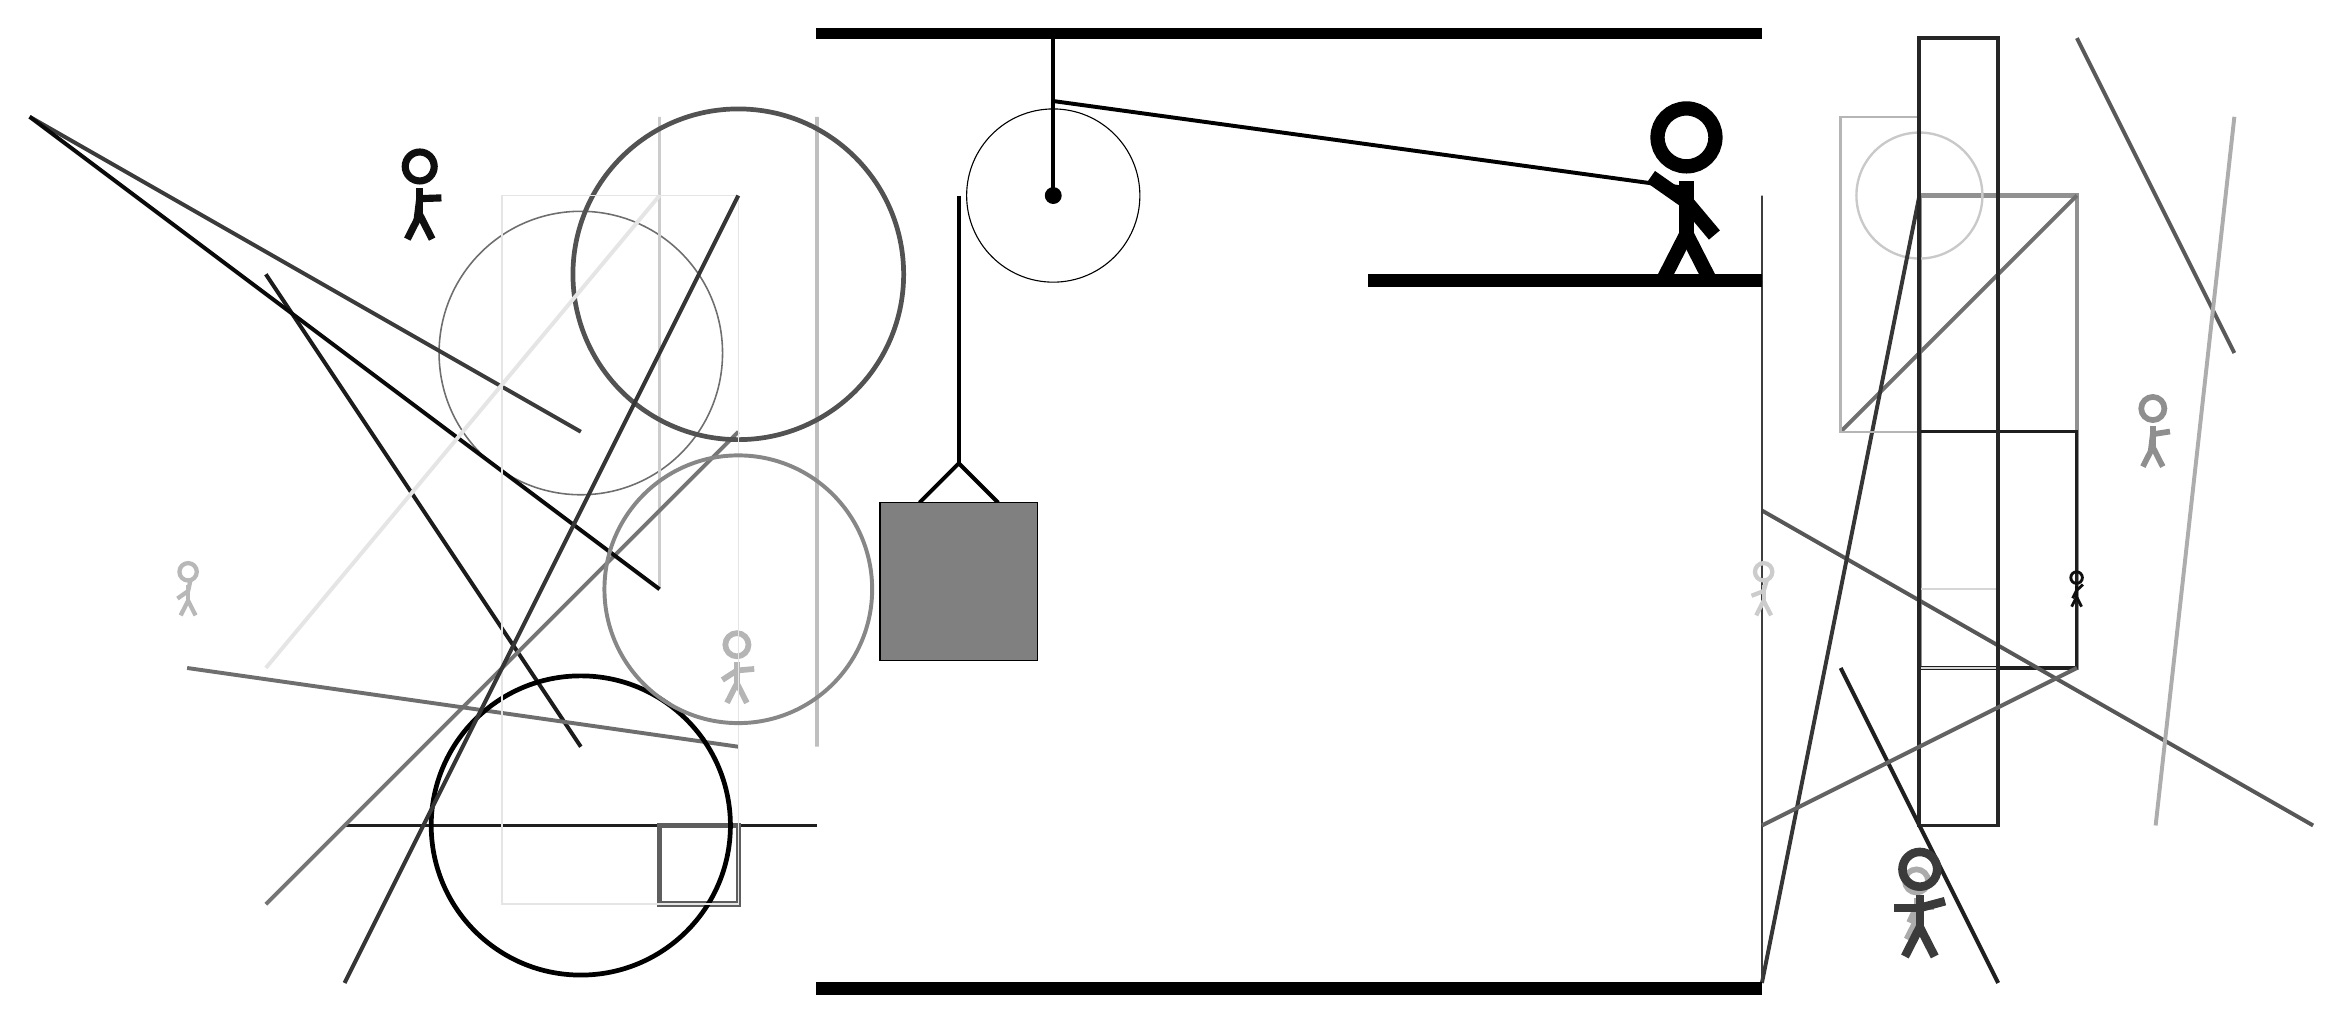
\begin{tikzpicture}
			%%%%% START %%%%%
			
			\draw[fill=black] (-2, 9) rectangle (10, 9.125);
			
			\draw [line width=0.2mm, color=black!57](-5, 5) circle (1.8);
			
			\draw[line width=0.4mm, color=black!20] (-4, 8) rectangle (-4, 2);
			\draw[line width=0.6mm, color=black!43] (12, 7) rectangle (14, 1);
			\draw[line width=0.5mm, color=black!77](-5, 4) -- (-12, 8);
			\draw[line width=0.5mm, color=black!25] (-2, 0) rectangle (-2, 8);
			
			\draw[line width=0.5mm, color=black!88](-2, -1) -- (-8, -1);
			
			\draw[line width=0.5mm, color=black!56](14, 7) -- (11, 4);
			
			\node[line width=0.5mm, color=black!44] at (15, 4) {\Strichmaxerl[4][83][9]};
			\node[line width=0.7mm, color=black!33] at (12, -2) {\Strichmaxerl[4][65][0]};
			\draw[line width=0.4mm, color=black!88] (12, 1) rectangle (14, 4);
			
			\node[line width=0.4mm, color=black!29] at (-3, 1) {\Strichmaxerl[4][33][5]};
			\draw[line width=0.5mm, color=black!89](-5, 0) -- (-9, 6);
			\draw[line width=0.3mm, color=black!16] (12, 1) rectangle (13, 2);
			\draw[line width=0.5mm, color=black!54](-3, 4) -- (-9, -2);
			\draw[line width=0.5mm, color=black!66](10, 3) -- (17, -1);
			\draw [line width=0.3mm, color=black!21](12, 7) circle (0.8);
			
			\draw[line width=0.5mm, color=black!88](13, -3) -- (11, 1);
			
			\draw[line width=0.5mm, color=black!79](10, -3) -- (12, 7);
			\draw[line width=0.3mm, color=black!76] (10, -3) rectangle (10, 7);
			\node[line width=0.6mm, color=black!94] at (-7, 7) {\Strichmaxerl[5][83][2]};
			\draw[line width=0.3mm, color=black!29] (12, 4) rectangle (11, 8);
			\draw [line width=0.6mm, color=black!68](-3, 6) circle (2.1);
			
			\draw[line width=0.5mm, color=black!85] (12, -1) rectangle (13, 9);
			\draw[line width=0.7mm, color=black!63] (-3, -2) rectangle (-4, -1);
			\draw[line width=0.5mm, color=black!57](-3, 0) -- (-10, 1);
			
			\draw[line width=0.5mm, color=black!65](14, 9) -- (16, 5);
			\draw [line width=0.6mm, color=black!100](-5, -1) circle (1.9);
			\draw[line width=0.5mm, color=black!96](-4, 2) -- (-12, 8);
			\node[line width=0.7mm, color=black!77] at (12, -2) {\Strichmaxerl[6][0][15]};
			\node[line width=0.2mm, color=black!28] at (-10, 2) {\Strichmaxerl[3][35][78]};
			\node[line width=0.4mm, color=black!20] at (10, 2) {\Strichmaxerl[3][21][74]};
			\draw[line width=0.2mm, color=black!10] (-3, -2) rectangle (-6, 7);
			\node[line width=0.3mm, color=black!94] at (14, 2) {\Strichmaxerl[2][63][43]};
			\draw [line width=0.5mm, color=black!47](-3, 2) circle (1.7);
			
			\draw[line width=0.5mm, color=black!61](10, -1) -- (14, 1);
			\draw[line width=0.5mm, color=black!79](-3, 7) -- (-8, -3);
			\draw[line width=0.5mm, color=black!10](-4, 7) -- (-9, 1);
			\draw[line width=0.5mm, color=black!32](15, -1) -- (16, 8);
			
			\draw (1, 7) circle (1.1);
			\draw[fill=black] (1, 7) circle (0.1);
			\draw[line width=0.5mm] (1, 9) -- (1, 7);
			
			\draw[line width=0.5mm](-0.7, 3.1) --  (-0.2, 3.6) -- (0.3, 3.1);
			\draw[fill=black!50] (-1.2, 3.1) rectangle (0.8, 1.1);
			
			\draw[line width=0.5mm](-0.2, 7) -- (-0.2, 3.6);
			\centerarc[line width=0.5mm](1, 7)(90:180:1.2000000000000002)
			\draw[line width=0.5mm](1, 8.2) -- (9, 7.1);
			
			\node at (9, 7) {\Strichmaxerl[10][-35][-50]};
			\draw[fill=black] (5, 6) rectangle (10, 5.85);
			
			\draw[fill=black] (-2, -3) rectangle (10, -3.15);
			
			%%%%% END %%%%%
		\end{tikzpicture}
	\end{figure}	
\end{document}